\documentclass[11pt]{article}
\usepackage[letterpaper,margin=1in]{geometry}
\usepackage{mytex}
\usepackage[colorlinks=true,linkcolor=blue,citecolor=blue]{hyperref}%

\usepackage{bookmark}

\usepackage{newtxtext, kotex}
\usepackage[all,cmtip]{xy}
\usepackage{tikz}
\usepackage{tikz-cd}
\usetikzlibrary{calc,positioning}

\usepackage{pgfplots}
\usepackage{caption}


\usepackage{fancyhdr}
%\fancyhf{} % sets both header and footer to nothing
\renewcommand{\headrulewidth}{0pt}


\usepackage[textwidth=1in,textsize=small,colorinlistoftodos]{todonotes} % todo 노트

\pagestyle{fancy}
\lhead{Myungsin Cho}
\chead{}
\rhead{}
%\rfoot{\date}

%Bibliography line spacing
% ADD THE FOLLOWING COUPLE LINES INTO YOUR PREAMBLE
\let\OLDthebibliography\thebibliography
\renewcommand\thebibliography[1]{
  \OLDthebibliography{#1}
  \setlength{\parskip}{0pt}
  \setlength{\itemsep}{0pt plus 0.3ex}
}

% section 폰트 바꿔주는거
\usepackage{titlesec}
\titleformat{\section}{\normalfont\large\center}{\thesection}{.5em}{}
\titleformat{\subsection}[runin]{\normalfont\bfseries}{\thesubsection}{.5em}{}

\newcommand{\yourname}{Myungsin Cho}

\newcommand{\univ}{Indiana University}

\newcommand\quelle[1]{{%
      \unskip\nobreak\hfil\penalty50
      \hskip2em\hbox{}\nobreak\hfil #1%
      \parfillskip=0pt \finalhyphendemerits=0 \par}}
      

\usepackage{amsmath,amsfonts,amssymb,mathrsfs}
\usepackage{amsthm,thmtools}
\newtheorem{theorem}{Theorem}
\newtheorem{proposition}{Proposition}
\newtheorem{lemma}{Lemma}
\newtheorem{corollary}[theorem]{Corollary}
\newtheorem*{goal}{Goal}
\newtheorem*{conjecture}{Conjecture}

\let\overto\xrightarrow
\title{Research Statement}
\author{Myungsin Cho}
\date{}
\begin{document}
\begin{center}\LARGE{Research Statement}\end{center}\vspace{.5em}
%\maketitle

My research investigates how ideas from algebraic topology reveal the structural relationships between algebra and arithmetic.
In particular, I use methods from stable homotopy theory to understand how duality, symmetry, and equivariant phenomena organize and connect seemingly distinct areas of mathematics.
My doctoral work contributed to leveraging arithmetic duality at the homotopical level, within the framework of algebraic K-theory.
More broadly, my research aims to develop conceptual and computational tools that show how homotopical structures govern both arithmetic and equivariant phenomena.

\section{Background}
One of the central aims of topology is to classify spaces according to appropriate notions of equivalence.  
The most rigid notion of sameness is that of a {\it homeomorphism}, a continuous map with its inverse.  
While this captures topological equivalence precisely, it is often too strict for understanding spaces up to deformation.  
{\it Homotopy theory} offers a more flexible perspective by identifying spaces that can be continuously deformed into one another, leading to the notion of a {\it homotopy type}.  
The resulting invariants, {\it homotopy groups} carry the deepest information: they completely determine the homotopy type, but are notoriously difficult to compute.

A guiding idea in {\it stable homotopy theory} is to study those properties of spaces that are preserved under iterated suspension:
\begin{figure}[h]
\centering
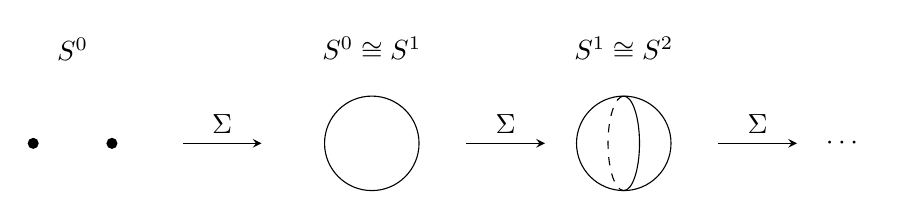
\begin{tikzpicture}[scale=1,>=stealth]

  % S^0: two points
  \node at (0,1.2) {$S^0$};
  \fill (-0.5,0) circle (2pt);
  \fill (0.5,0)  circle (2pt);

  % arrow to S^1
  \draw[->] (1.4,0) -- (2.4,0) node[midway,above] {$\Sigma$};

  % S^1: circle
  \node at (3.8,1.2) {$\SI S^0 \cong S^1$};
  \draw (3.8,0) circle (0.6);

  % arrow to S^2
  \draw[->] (5,0) -- (6,0) node[midway,above] {$\Sigma$};

  % S^2: sphere (projected)
  \node at (7.0,1.2) {$\SI S^1 \cong S^2$};
  \draw (7.0,0) circle (0.6);
  \draw (7.0,-0.6) arc (-90:90:0.2 and 0.6);
  \draw[dashed] (7.0,0.6) arc (90:270:0.2 and 0.6);

  % arrow to dots
  \draw[->] (8.2,0) -- (9.2,0) node[midway,above] {$\Sigma$};

  % dots ...
  \node at (9.8,0) {$\cdots$};

\end{tikzpicture}
\captionsetup{font=footnotesize}
\caption{
Iterated suspensions $\SI^n S^0 \cong S^n$ of spheres.
}
\end{figure}

In particular, the {\it Freudenthal suspension theorem} shows that the homotopy classes of maps $[X,Y]$ stabilize after finitely many suspensions, providing a linear approximation to homotopy theory itself.
\begin{figure}[h]
\centering
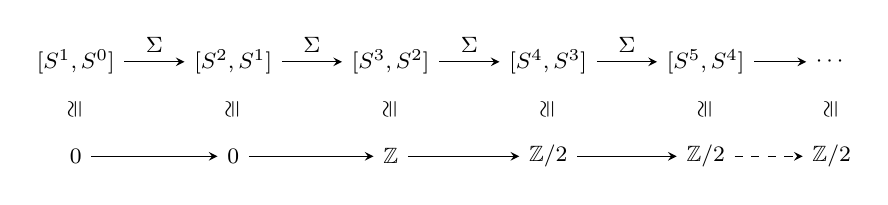
\begin{tikzpicture}[>=stealth, every node/.style={font=\footnotesize}]
  % Top row: homotopy classes
  \node (c0) at (0,0.6) {$[S^1,S^0]$};
  \node (c1) at (2.0,0.6) {$[S^2,S^1]$};
  \node (c2) at (4.0,0.6) {$[S^3,S^2]$};
  \node (c3) at (6.0,0.6) {$[S^4,S^3]$};
  \node (c4) at (8.0,0.6) {$[S^5,S^4]$};
  \node (c5) at (9.6,0.6) {$\cdots$};

  % Bottom row: resulting groups
  \node (v0) at (0,-0.6) {$0$};
  \node (v1) at (2.0,-0.6) {$0$};
  \node (v2) at (4.0,-0.6) {$\mathbb{Z}$};
  \node (v3) at (6.0,-0.6) {$\mathbb{Z}/2$};
  \node (v4) at (8.0,-0.6) {$\mathbb{Z}/2$};
  \node (v5) at (9.6,-0.6) {$\mathbb{Z}/2$};

  % Horizontal arrows (homotopy classes)
  \draw[->] (c0) -- (c1) node[midway,above] {$\Sigma$};
  \draw[->] (c1) -- (c2) node[midway,above] {$\Sigma$};
  \draw[->] (c2) -- (c3) node[midway,above] {$\Sigma$};
  \draw[->] (c3) -- (c4) node[midway,above] {$\Sigma$};
  \draw[->] (c4) -- (c5);

  % Horizontal arrows (values)
  \draw[->] (v0) -- (v1);
  \draw[->] (v1) -- (v2);
  \draw[->] (v2) -- (v3);
  \draw[->] (v3) -- (v4);
  \draw[dashed,->] (v4) -- (v5);

  % Rotated isomorphisms
  \foreach \i in {0,1,2,3,4}{
    \node at ($(c\i)!0.5!(v\i)$) {\rotatebox{90}{$\cong$}};
  }
  \node at ($(c5)!0.5!(v5)$) {\rotatebox{90}{$\cong$}};

  % Annotation
%  \node[right=1pt of v5] {\scriptsize (stabilized value)};
\end{tikzpicture}
\captionsetup{font=footnotesize}
\caption{
The sequence $0 \to 0 \to \mathbb{Z} \to \mathbb{Z}/2 \to \cdots$ stabilizes at $\mathbb{Z}/2$, illustrating the suspension theorem in a concrete case.
}
\end{figure}

Suspensions of homotopy groups eventually stabilize after finitely many iterations, and this stabilization provides the linear approximation described by Freudenthal’s theorem.
In this stabilized setting, new patterns and algebraic structures emerge, making it possible to study homotopical phenomena that were previously too complex to handle directly.
This shift—from spaces to stable homotopy types—establishes a framework in which algebraic and homotopical ideas can be applied in a unified way, forming the foundation of modern algebraic topology.

Much of my work takes place within this stable framework, where duality, symmetry, and equivariant structures reveal deep connections between algebra and topology.

\section{Current research and direction}
Building on the framework of stable homotopy theory, my current research explores how algebraic and homotopical ideas interact across several fronts—particularly through {\it algebraic K-theory}, {\it equivariant algebra}, and their connections to number theory and combinatorics.
Rather than treating these areas in isolation, I study how organizing principles such as duality, symmetry, and operadic compatibility arise in parallel forms across them.
The following sections describe how these themes manifest in my recent and ongoing work.


\subsection{Algebraic K-theory and Arithmetic Duality.}
My dissertation investigates how duality phenomena from number theory manifest in algebraic K-theory.
In arithmetic geometry, a central duality known as {\it Tate–Poitou duality} describes relationships between the cohomology of number rings and their completions. 
A natural question is whether an analogous duality exists in algebraic K-theory.

The case at the prime $2$ had remained open since the work of Blumberg and Mandell \cite{MR4121155}. 
They proved the duality for all odd primes but left the even-prime case conjectural due to the essential role of real embeddings and the resulting technical complications.
My dissertation resolves this case, establishing a K-theoretic version of Tate–Poitou duality at the prime $2$.

\begin{theorem}[\cite{Cho}]
Let $F$ be a number field.
There is a canonical weak equivalence between  the {\it homotopy fiber of the completion map} $\ka$ in $K(1)$-local algebraic K-theory$\colon$
\[\ka\colon L_{K(1)}K(\calO_F[\tfrac{1}{2}]) \longrightarrow \prod_{\nu \mid 2} L_{K(1)}K(F_\nu^\w)\]
and the $\bZ_2$-Anderson dual of the algebraic K-theory of $\calO_F[\tfrac{1}{2}]\colon$
 \begin{equation}\label{fib}
 \Fib(\ka) \simeq \SI^{-1} I_{\bZ_2} L_{K(1)}K(\calO_F[\tfrac{1}{2}]).
\end{equation}
\end{theorem}

This equivalence can be viewed as a homotopical counterpart of classical Artin-Verdier duality.
Figure~\ref{fig:duality} illustrates how the arithmetic and homotopical dualities align, connected through the Thomason descent spectral sequence.
\begin{figure}[h]
\centering
\begin{tikzcd}[column sep=4em, row sep=2em]
  \textbf{\small Arithmetic duality:}
    \arrow[d, decorate, decoration={snake, amplitude=0.3mm, segment length=2.5mm}, 
           "\text{\footnotesize Thomason SS}" right]
    &
  {H^s_{\textup{\'et}}\!\big(\calO_F[\tfrac{1}{p}];\,\bZ/p^k(\tfrac{t}{2})\big)}
    \arrow[d, Rightarrow]
    \arrow[rr, leftrightarrow, "\text{\footnotesize Pontryagin dual}"]
    &&
  {H^{3-s}_c\!\big(\calO_F[\tfrac{1}{p}];\,\bZ/p^k(-\tfrac{t}{2})\big)}
    \arrow[d, Rightarrow] \\[1ex]
  \textbf{\small Homotopical duality:}
    &
  {L_{K(1)}K(\calO_F[\tfrac{1}{p}])}
    \arrow[rr, leftrightarrow, "\text{\footnotesize Anderson dual}"]
    &&
  {\Fib(\kappa)}
\end{tikzcd}
\captionsetup{font=footnotesize, skip=0em}
\caption{
Arithmetic and homotopical dualities in parallel,
linked by the Thomason descent spectral sequence.
}
\label{fig:duality}
\end{figure}

An immediate consequence of this theorem gives new insight into the algebraic K-theory of the {\it sphere spectrum} $\bS$.
Using the case $F=\bQ$ together with {\it trace methods}, one obtains the following result.

\begin{corollary}[\cite{Cho}]
Let $\ta_\bS\colon K(\bS)_2^\w \to TC(\bS)_2^\w$ be the $2$-completed cyclotomic trace map for the sphere spectrum.
After taking connective covers, the homotopy fiber $\Fib(\ta_\bS)$ is canonically weakly equivalent to the $\bZ_2$-Anderson dual of $L_{K(1)}K(\bZ)\colon$
\[\Fib(\ta_\bS)[0,\infty) \simeq \Sigma^{-1} I_{\bZ_2}\, L_{K(1)}K(\bZ)[0,\infty).\]
\end{corollary}
Together, these results provide concrete computational tools for the $2$-primary algebraic K-theory of $\bS$, clarifying how the homological behavior of the integers is reflected in stable homotopy theory through algebraic K-theory.

Beyond computation, this work relates to several active areas in arithmetic and homotopy theory.
The homotopy fiber $\Fib(\kappa)$ appearing in the duality theorem connects to objects such as the $p$-adic Langlands correspondence \cite{MR2905536} and compactly supported K-theory \cite{MR3211458}.
By giving a precise homotopical description of $\Fib(\kappa)$, this work provides a foundation for exploring how these structures interact across arithmetic geometry and higher algebra.

Overall, this research develops new methods in $2$-primary algebraic K-theory that clarify the structure of number rings and point toward broader extensions in arithmetic topology.

\subsection{Equivariant algebras and homotopical combinatorics.}
My research in equivariant algebras investigates how combinatorial structures capture and control  operations arising in equivariant stable homotopy theory.
A central organizing idea is the notion of a {\it transfer system} \cite{MR4244201}, which encodes which “transfer” maps between subgroups are allowed, subject to natural coherence conditions such as compatibility with conjugation and restriction.
For example, in the case of the cyclic group $C_{p^2}$, the possible transfer systems are shown in Figure~\ref{fig:transferCp2}.
\begin{figure}[h]
\centering
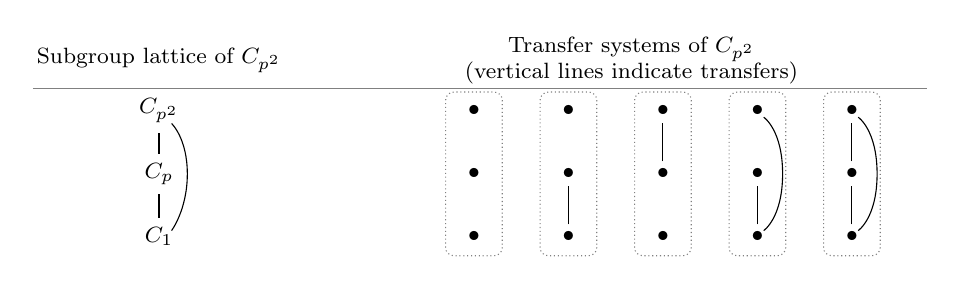
\begin{tikzpicture}[scale=.8, every node/.style={font=\footnotesize}]
  % Titles
  \node at (0,2.8) {Subgroup lattice of $C_{p^2}$};
  \node[align=center] at (7.5,2.8)
    {Transfer systems of $C_{p^2}$\\ \footnotesize(vertical lines indicate transfers)};

  % --- 구분선 ---
  \draw[gray, thin] (-2,2.35) -- (12.2,2.35);

  % === Left: subgroup lattice ===
  \node (C1)  at (0,0)   {$C_{1}$};
  \node (Cp)  at (0,1.0) {$C_{p}$};
  \node (Cp2) at (0,2.0) {$C_{p^2}$};

  \draw (C1) -- (Cp);
  \draw (Cp) -- (Cp2);
  \draw plot [smooth, tension=1.2] coordinates {(0.2,0.1) (0.45,1.0) (.2,1.8)};

  % === Right: five transfer systems ===
  % x: 5.0, 6.5, 8.0, 9.5, 11.0 / y: 0, 1, 2
  % (각 기둥을 먼저 박스로 감싸기 위해 박스부터 그림)
  \foreach \x in {5.0,6.5,8.0,9.5,11.0}{
    \draw[gray!100, densely dotted, rounded corners=3pt]
      (\x-0.45,-0.3) rectangle (\x+0.45,2.3);
  }

  % (1) isolated dots
  \node at (5.0,0) {$\bullet$}; \node at (5.0,1) {$\bullet$}; \node at (5.0,2) {$\bullet$};

  % (2) bottom–middle
  \node at (6.5,0) {$\bullet$}; \node at (6.5,1) {$\bullet$}; \node at (6.5,2) {$\bullet$};
  \draw (6.5,0.2) -- (6.5,0.8);

  % (3) middle–top
  \node at (8.0,0) {$\bullet$}; \node at (8.0,1) {$\bullet$}; \node at (8.0,2) {$\bullet$};
  \draw (8.0,1.2) -- (8.0,1.8);

  % (4) full chain
  \node at (9.5,0) {$\bullet$}; \node at (9.5,1) {$\bullet$}; \node at (9.5,2) {$\bullet$};
  \draw (9.5,0.2) -- (9.5,0.8);
  \draw plot [smooth, tension=1.4] coordinates {(9.6,0.1) (9.9,1.0) (9.6,1.9)};

  % (5) chain + curved bottom–top
  \node at (11.0,0) {$\bullet$}; \node at (11.0,1) {$\bullet$}; \node at (11.0,2) {$\bullet$};
  \draw (11.0,0.2) -- (11.0,0.8);
  \draw (11.0,1.2) -- (11.0,1.8);
  \draw plot [smooth, tension=1.4] coordinates {(11.1,0.1) (11.4,1.0) (11.1,1.9)};
\end{tikzpicture}
\captionsetup{font=footnotesize} % ← 캡션 크기 줄이기
\caption{Subgroup lattice of the cyclic group $C_{p^2}$ of order $p^2$  (left) and its five distinct transfer systems (right). These five systems classify, up to homotopy, the $N_\infty$-operads for $C_{p^2}$.}
\label{fig:transferCp2}
\end{figure}

Transfer systems provide a combinatorial model for the algebraic structure underlying genuine equivariant commutative ring spectra, encoded by {\it Tambara functors} \cite{MR1209937}.
Their additive (transfer) and multiplicative (norm) operations are governed by a pair of transfer systems satisfying a compatibility condition, forming a {\it compatible pair}.
In collaboration with David Chan, David Mehrle, Pablo Sanchez Ocal, Angelica Osorno, Ben Szczesny, and Paula Verdugo, we study the correspondence between such combinatorial data and the {\it pairings of $N_\infty$-operads} \cite{MR2544392} that model these operations.
Constructing these pairings is subtle even non-equivariantly, and our results give the first systematic framework for realizing them in the genuine equivariant setting.

\begin{theorem}[\cite{CCM+}]
An action of one $N_\infty$-operad on another implies that their associated transfer systems form a compatible pair.
If a compatible pair of transfer systems has a complete additive component, then there exists a pairing of $N_\infty$-operads that realizes it.
\end{theorem}

Motivated by this result, we conjecture that the correspondence between compatible pairs and operadic pairings holds in full generality:
\begin{conjecture}
 For every finite group $G$, every compatible pair of $G$-transfer systems should be realizable by some pairing of $N_\infty$-operads.
\end{conjecture}

Establishing this equivalence would complete the conceptual bridge between the combinatorial and homotopical descriptions of incomplete Tambara functors and provide a combinatorial classification of admissible equivariant multiplicative structures.


Building on this framework, we have proved several further realizability results that support this conjecture.
For instance, the transfer systems associated to the {\it equivariant linear isometries} and {\it Steiner operads} are realized by the corresponding pairing of operads, and $J$-local transfer systems $(\mathcal{T}_J,\mathcal{T}_J)$ are likewise realizable for any subgroup $J\le G$.
Moreover, we introduce a general construction principle showing that whenever two {\it intersection monoids} $M$ and $N$ admit a pairing $\xi\colon M\times N\to N$, one obtains a corresponding pairing of operads $(\mathcal{O}^{\vee}(M),\mathcal{O}^{\vee}(N))$.

Together, these results form the first systematic framework for classifying compatible transfer system pairs and understanding how combinatorial and homotopical perspectives on equivariant algebra align.
They provide a computable foundation for studying incomplete Tambara functors and genuine equivariant ring spectra, and illustrate how ideas from combinatorics and operad theory drive new advances in equivariant homotopy theory.


\subsection{Real algebraic K-theory and homological trace methods.}
Real algebraic K-theory offers a framework for studying algebraic structures equipped with involutive symmetries, combining topological and arithmetic ideas.
Introduced by Hesselholt and Madsen \cite{HMreal}, it assigns {\it genuine $C_2$-equivariant spectra} to rings with an {\it anti-involution}.
This theory refines and unifies classical algebraic K-theory, Hermitian K-theory, and $L$-theory by incorporating this additional symmetry.

In collaboration with Teena Gerhardt, Liam Keenan, Juan Moreno, and J.D. Quigley, we are extending the {\it homological trace methods} developed by Bruner and Rognes \cite{MR2153113} to the $C_2$-equivariant setting.
Our work constructs a new spectral sequence based on $RO(C_2)$-graded homology, providing computational access to invariants in real algebraic K-theory.
\begin{theorem}[Gerhardt--C.--Keenan--Moreno--Quigley]
 For a $C_2$-equivariant $\ef$-ring spectrum $R$ with twisted $\bT$-action, there is a natural $\aA_\star^{C_2}$-comodule algebra spectral sequence of Mackey functors$\colon$
 \[E^2_{\ast,\star} = H^{-\ast}(B_{C_2}\bT; H \ul{\bF_2}_\star (R)) \Rightarrow H\ul{\bF_2}_\star^c (R^{h_{C_2}\bT})\]
\end{theorem}
This construction provides the first homological tool for accessing real algebraic K-theory, extending classical trace methods while incorporating genuine $C_2$-equivariance.

Our approach builds on recent advances in {\it real trace methods}, which adapt topological Hochschild and cyclic homology to the $C_2$-equivariant context \cite{Dotto,Hogenhaven}.
Extending the homological approach of Bruner and Rognes to this setting yields new computational methods for studying equivariant invariants and new approximations for important spectra such as the {\it real bordism spectrum} $MU_\bR$.

The long-term goal of this project is to apply these techniques to analyze the real algebraic K-theory of fundamental spectra including $MU_\bR$ and the {\it real Brown--Peterson spectrum} $BP_\bR$.
In particular, we aim to establish a {\it real analogue of the Segal conjecture} for these spectra, which would parallel one of the most powerful computational results in classical topology and provide new insights into how symmetry shapes algebraic K-theory at chromatic height 1 and beyond.

% 아카이브에 페이퍼 올라올 시
%\textbf{Analytic Stacks and Hyperbolicity.}
%In a parallel project with Geonhee Cho, we develop a stack-theoretic extension of the Green–Griffiths–Demailly (GGD) method for studying Brody hyperbolicity via jet differentials on compact analytic Deligne–Mumford stacks.
%Our framework provides a unified analytic setting encompassing both complex manifolds and orbifold quotients while preserving the asymptotic behavior of Green–Griffiths bundles.
%This work, now available as a preprint, lays the analytic groundwork for a broader program aimed at extending hyperbolicity to higher and derived stacks.

\section{Future research direction}
My future research builds directly on my current work, extending results on duality phenomena in algebraic K-theory and advancing the foundations of equivariant algebra. 
A central aim is to further develop the connections between homotopical methods, arithmetic dualities, and symmetry in algebraic and geometric contexts.

I am particularly interested in exploring links to complex and derived geometry, where tools from algebraic K-theory and equivariant homotopy theory may reveal new relationships between curvature, symmetry, and cohomological phenomena. 
This direction naturally extends the analytic and homotopical aspects of my research, bridging ideas from topology and geometry.

In parallel, I plan to develop projects that emphasize concrete computations and examples, especially in areas such as homotopical combinatorics and topological data analysis. 
These topics are well suited for undergraduate involvement and provide natural entry points into algebraic topology. 
I view cultivating such accessible research directions as an essential part of advancing the field and training the next generation of mathematicians.

\subsection*{Duality and Symmetry in Algebraic K-theory}
Building on my work on K-theoretic Tate–Poitou duality, I plan to extend these ideas in several directions: higher-dimensional analogues, chromatic refinements, and new formulations in the real algebraic K-theory setting.

A first line of investigation concerns higher-dimensional analogues of the K-theoretic duality.
While progress has been made for odd primes \cite{Braunling}, the higher-dimensional case at the prime 2 remains open.
Building on the techniques I developed to address the unique challenges of the prime 2 setting, I aim to extend these results to this remaining case.

These arithmetic extensions naturally connect to chromatic phenomena in stable homotopy theory.
Recent results \cite{HRW} suggest that the connective Adams summand $l$ behaves in ways analogous to local rings in arithmetic geometry.
Motivated by this analogy, I plan to develop a chromatic analogue of arithmetic duality, formulating a K-theoretic duality at higher chromatic heights.

Finally, I aim to pursue these ideas within the framework of real algebraic K-theory.
An ultimate goal is to construct a {\it real Thomason spectral sequence}, providing a systematic computational tool for the theory.
This will require developing a genuine equivariant version of \'etale cohomology for commutative ring spectra, followed by adapting classical descent spectral sequence techniques to the $C_2$-equivariant setting.
Such a construction would parallel Thomason’s spectral sequence in the classical case and offer a new computational approach to real algebraic K-theory.


\subsection*{Foundations for Equivariant Algebra}
A key direction of my future work is to develop the basic algebraic framework underlying equivariant stable homotopy theory.
While advanced constructions such as Tambara functors capture much of the structure, many of the elementary notions familiar from commutative algebra remain to be formulated in the equivariant setting.

A natural entry point is the study of commutative $G$-rings, a simpler type of equivariant algebraic object that Tambara functors generalize.
Even in this case, elementary concepts such as algebraic extensions and algebraic closures exhibit subtle equivariant pathologies.
Investigating these questions offers an accessible entry point that also exposes conceptual obstructions in the more general theory of Tambara functors.
Beginning with these manageable cases allows one to develop the algebraic intuition and categorical techniques needed to approach the full equivariant framework.

My goal is to establish such foundational concepts and structures within the equivariant setting.
This foundational program would provide the analogue of commutative algebra for equivariant algebraic geometry, bridging the gap between algebraic and homotopical formulations of equivariant descent.

\subsection*{Analytic Stacks and Hyperbolicity}
Another direction of my research concerns the study of {\it hyperbolicity} in the setting of stacks.
In complex geometry, hyperbolicity captures rigidity and asymptotic constraints on holomorphic maps, and recent work by Borghesi and Tomassini \cite{MR3673667} has extended these ideas to {\it stacks} and {\it simplicial presheaves}, showing that they admit meaningful formulations beyond complex manifolds.

Together with Geonhee Cho, I am developing a stack-theoretic extension of the {\it Green–Griffiths–Demailly} method for studying Brody hyperbolicity via jet differentials on compact analytic {\it Deligne–Mumford stacks}.
This project establishes an analytic foundation that unifies the treatment of hyperbolicity for complex manifolds and orbifold quotients and serves as a first step toward formulating hyperbolicity for higher and derived stacks.

Building on this framework, we aim to extend the theory to derived and higher stacks, constructing explicit examples that illustrate how rigidity and curvature behave in these generalized settings.
Ultimately, this work connects classical analytic geometry with modern homotopical and stack-theoretic methods, uncovering new interactions between symmetry, deformation, and geometric structure.

\subsection*{Undergraduate Research Directions}
Several aspects of my work give rise to problems and projects that are accessible at an undergraduate level yet remain closely connected to broader research questions.
Two areas in particular, combinatorial transfer systems and topological data analysis (TDA), offer tractable problems that both engage students and contribute to the development of my research programs.

One direction is the study of {\it transfer systems} from a combinatorial perspective.
Transfer systems are defined directly in terms of subgroup lattices, making them elementary to describe while still encoding the algebraic constraints that govern equivariant operations.
Counting and classifying finite posets associated with transfer systems not only provides combinatorial insight but also informs the structural classification of $N_\infty$-operads and Tambara functors, clarifying how discrete data control admissible algebraic operations.
This line of investigation illustrates how even elementary combinatorics can feed directly into ongoing developments in equivariant algebra.

Another area is {\it topological data analysis} (TDA), which applies algebraic topology to study the structure of high-dimensional data sets.
Methods such as {\it persistent homology} can be introduced in a visual and computationally accessible way, yet they lead naturally into deeper questions about stability, functoriality, and the role of cohomology operations.
These connections remain an active area of research, and concrete case studies in TDA provide a natural testing ground for exploring how homotopical invariants can yield new insights into the shape and geometry of data.

In this way, projects in combinatorics and data science serve not only as entry points for undergraduate participation but also as stepping stones toward more advanced problems aligned with my core research agenda.

\section{Conclusion}
At the heart of my research lies the perspective of {\it stable homotopy theory}—a framework in which topology, algebra, and geometry meet on equal footing.
Within this setting, ideas such as duality, symmetry, and equivariance reveal how seemingly distinct structures reflect the same underlying homotopical patterns.
My work develops this viewpoint to expose the shared logic that links arithmetic, combinatorics, and topology.

Looking ahead, I aim to expand this program by using stable homotopy theory as a unifying language for understanding duality and symmetry across mathematical contexts.
A central goal is to build conceptual and computational tools—within algebraic K-theory, equivariant homotopy theory, and beyond—that clarify how these structures behave and interact.
Equally important is keeping this program accessible: developing problems that invite undergraduate participation and creating avenues for collaboration across levels of expertise.

In this sense, my research advances not only the technical reach of stable homotopy theory but also its role as a common ground where diverse mathematical ideas can meet, evolve, and inspire new connections.

\bibliography{RS_bib}
\bibliographystyle{alphaurl}

\end{document}